%!TEX root = ./../main.tex
\section{Streaming-Data}

Das Ziel unserer Aufgabenstellung ist die Verarbeitung von Streaming-Daten in Echtzeit. Die Streaming-Data-Architektur
von Psaltis \cite{psaltis2017streaming} ist für diese Art von Problem konzipiert und bildet die Grundlage für
unsere Architektur. Nach der kurzen Vorstellung der Streaming-Data-Architektur von Psaltis, zeigen wir unsere eigene konkrete
Umsetzung und vergleichen eingesetzten Technologien mit Alternativen.

\subsection{Streaming-Data-Architektur nach Psaltis}

In Abbildung \ref{fig:streaming_data_architecture-psaltis} sind die Komponenten der Streaming-Data-Architektur, wie Psaltis \cite{psaltis2017streaming}
sie entwickelt hat, abgebildet. Der Collection-Tier ist der Einstiegspunkt, der Daten in das System bringt. Unabhängig von dem verwendeten
Protokoll, werden die Daten mithilfe eines dieser Patterns übertragen \cite{psaltis2017streaming}:
\begin{itemize}
    \item Request/response pattern
    \item Publish/subscribe pattern
    \item One-way pattern
    \item Request/acknowledge pattern
    \item Stream pattern
\end{itemize}

Bei der Datenquelle kann es sich sowohl um von Hardware und auch von Software generierte Events handeln. Beispiele hierfür sind
Temperatur, Lautstärke oder auch Browser-Clicks.


\begin{figure*}
    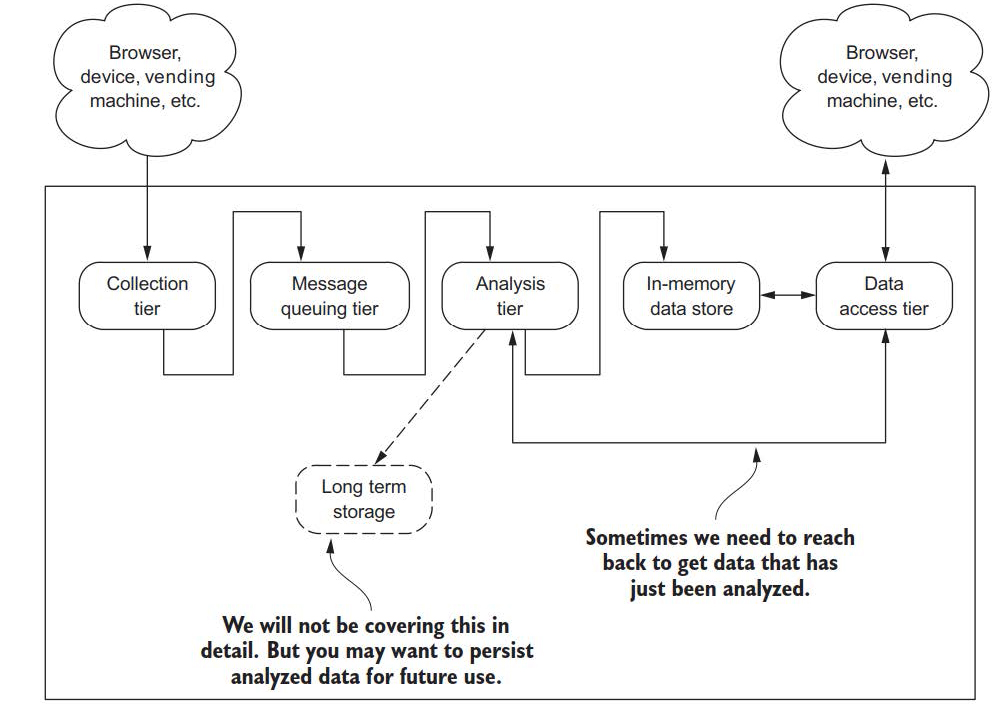
\includegraphics[width=\textwidth]{images/streaming_data_architecture-psaltis.jpg}
    \caption{Streaming-Data-Architektur \cite{psaltis2017streaming}}
    \label{fig:streaming_data_architecture-psaltis}
\end{figure*}


Um die Daten vom Collection-Tier auf den Rest der Pipeline zu verteilen wird ein Messaging Queuing Tier implementiert.
Das Message-Queuing-Model ist ein Modell zur Interprozesskommunikation. Anwendungen schicken
Nachrichten an eine Nachrichtenschlange, von der andere Anwendungen diese abholen können \cite{gray2003interprocess}.
Dadurch werden die eingesetzten Systeme voneinander entkoppelt und die Kommunikation findet nicht durch direkte Aufrufe,
sondern über die Queue statt \cite{psaltis2017streaming}. Im vorliegenden Fall wird der Collection-Tier vom Rest der Pipeline entkoppelt.

Im Analysis-Tier werden auf die Streams des Message-Queuing-Tiers kontinuierlich Queries angewandt um Muster in den Daten zu erkennen.
Hier können Event-Stream-Processing-Systeme (ESP) wie z.\,B. Apache Flink, Apache Spark oder Apache Storm oder
auch Complex-Event-Processing-Systeme (CEP) wie z.\,B. Esper oder Apache Samza eingesetzt werden \cite{psaltis2017streaming}.
In ESP wird die Verarbeitungslogik imperativ umgesetzt, wohingegen CEP einen deklarativen Ansatz verfolgt.
Die Event-Processing-Languages (EPL) sind Sprachen, die über Sequenz-, Konjunktions-, Disjunktions- und Negationsoperatoren
verfügen und für CEP entwickelt wurden \cite{hedtstck2017complex}. Als Basis der Operatoren werden Windows eingesetzt.
Ist die Analyse vorbei und die Ergebnisse stehen fest, können die Ergebnisse verworfen werden, zurück in die Streaming-Plattform gespeichert werden,
für eine Echtzeitnutzung oder die Stapelverarbeitung gespeichert werden \cite{psaltis2017streaming}. Wie der Abbildung \ref{fig:streaming_data_architecture-psaltis}
zu entnehmen ist, schlägt Psaltis hierfür eine In-Memory-Datenbank (IMDB), einen Data-Access-Tier und ein Long-Term-Storage vor.
Je nach Anwendungsfall ist das eine System dem anderen überlegen.

\subsection{Unsere Streaming-Data-Architektur}
In diesem Kapitel geht es um die Frage, welche Technologie wir in dem jeweiligen Tier einsetzen und wieso wir uns dafür entschieden haben.
Technische Details, die die Implementierung betreffen, erläutern wir im nächsten Kapitel.
%TODO: Quellen zu den einzelnen Punkten/Systemen
\begin{itemize}
    \item \textit{Collection-Tier.} Als Datenquelle nutzen wir die frei zugänglichen Daten von Wikipedia. Konkret handelt es sich um die Recent-Changes,
    also die aktuellen Änderungen an Wikipedia-Einträgen. Details hierzu sind im nächsten Kapitel beschrieben. Wir entschieden uns für Wikipedia als
    Datenquelle, weil es eine offene Plattform ist, die einen freien Zugang zu allen Daten gibt.

    \item \textit{Messaging-Queuing-Tier.} Wir nutzen Kafka als Messaging-System, weil es skalierbar ist, einen hohen Datendurchsatz ermöglicht,
    Real-Time-Messaging unterstützt, eine einfache Client-Anbindung ermöglicht und Events standardmäßig persistiert \cite{chellappan2018practical}. Der letzte Punkt ist
    besonders relevant, da für die Entwicklung der Regeln eine statische Datenmenge einfacher zu handhaben ist.

    \item \textit{Analysis-Tier.} Die Analyse der Wikipedia-Edit-Events sollte deklarativ erfolgen. Dadurch erhofften wir uns
    in kurzer Zeit eine Vielzahl an Regeln zu testen und so ein gutes Verständnis für die Daten zu erhalten. Aufgrund dieser Vorgabe
    entschieden wir uns für Esper. Es bietet eine CEP-Implementierung, die nach einem regelbasierten Ansatz -- somit deklarativ -- arbeitet.
    Ein weiterer Punkt, der für Esper sprach, war zum einen die Esper Processing Language und die Implementierung der Anwendung in Java.

    \item \textit{In-Memory-Data-Store, Long-Term-Storage und Data-Access-Tier.} Für diese drei Komponenten haben wir selbst keine Implementierung vorgesehen.
    Im Ausblick geben wir hierzu Ideen zu möglichen Weiterentwicklungen.
\end{itemize}